\section{Ejercicios}
\subsection{main.html}
Cree un archivo main.html:
Creamos un archivo main.html , el cual llamara a los archivos  javascript , el archivo p5.min.js es una librería para gráfícos.En el archivo kdtree.js se encontrara la estructura ,mientras que en sketch.js prepara el ambiente de trabajo donde haremos las pruebas .
\begin{lstlisting}[language=c++,
                   directivestyle={\color{black}}
                   emph={int,char,double,float,unsigned},
                   emphstyle={\color{blue}}
                  ]
<html >
<head >
<title >Kd tree </ title >
<script src ="p5.min.js" ></ script >
<script src =" kdtree.js" ></ script >
<script src =" sketch.js" ></ script >
</head >
<body >
</body >
</html >
\end{lstlisting}

\begin{figure}[H]
  \centering
  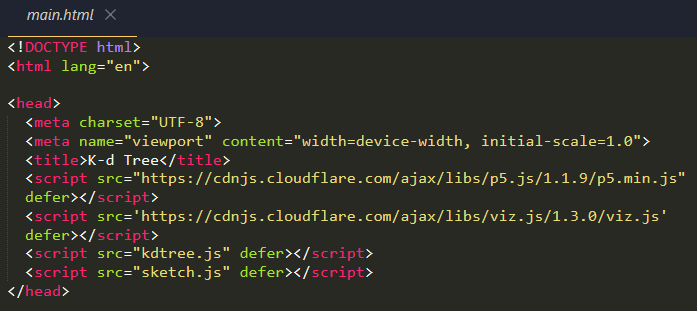
\includegraphics[width=1\textwidth]{images/uno.PNG}
  \caption{main.html}
  \label{fig:act-1}
\end{figure}

